\documentclass[11pt]{report}

\usepackage{fullpage} % Package to use full page
\usepackage{parskip} % Package to tweak paragraph skipping
\usepackage{tikz} % Package for drawing
\usepackage{amsmath}
\usepackage{amsfonts}
\usepackage{float}
\usepackage{hyperref}
\usepackage[utf8]{inputenc}  
\usepackage[T1]{fontenc}       
\usepackage[dvipsnames]{xcolor}
\usepackage{fancyhdr} % Required for custom headers
\usepackage{lastpage} % Required to determine the last page for the footer
\usepackage{extramarks} % Required for headers and footers
\usepackage[usenames,dvipsnames]{color} % Required for custom colors
\usepackage[labelformat=parens,labelsep=quad,skip=3pt]{caption}
\usepackage{subcaption}
\usepackage[makeroom]{cancel}
\usepackage{graphicx} % Required to insert images
\usepackage{listings} % Required for insertion of code
\usepackage{courier} % Required for the courier font
\usepackage{lipsum} % Used for inserting dummy 'Lorem ipsum' text into the template
\usepackage[ruled,vlined]{algorithm2e}

\newcommand{\HRule}{\rule{\linewidth}{0.5mm}}


% % % % % % % % % % 
% COMMANDE NOMBRE DE FRAGMENTS
% % % % % % % % % % 
\newcommand\xfrag{3150 }
% % % % % % % % % % 
% COMMANDE NOMBRE DE PAPYRI
% % % % % % % % % % 
\newcommand\xpapy{46 }

\begin{document}

\pagenumbering{gobble}

% % % % % % % % % % 
% PAGE DE GARDE
% % % % % % % % % % 

\begin{titlepage}
  \begin{center}

    % Upper part of the page. The '~' is needed because \\
    % only works if a paragraph has started.

    % Title
    \HRule \\[0.4cm]
    { \Huge \textbf{Papyrus matching using machine learning}\\[0.4cm] }
    \HRule \\[0.8cm]
    
    {\Large \textbf{Pierre-Loup \textsc{Nicolas}}\\[0.2cm]
     \textit{Supervisors:} Raphaël \textsc{Marée}, Pierre \textsc{Geurts}\\[1cm]}
    
    
\includegraphics[scale=0.25]{uliege2.png}~\\[1.3cm]
    
    {\huge Thesis submitted for the degree of\\
    \textsc{MSc in Data Science}}
    \\[3cm]

    % Bottom of the page
    {\Large University of Liège\\
    Faculty of Applied Science}\\[0.2cm]
    {\large Academic year 2019 — 2020}

  \end{center}
\end{titlepage}

% % % % % % % % % % 
% ABSTRACT
% % % % % % % % % % 

\vspace*{5cm}
{\Huge \textbf{Abstract}}\\[0.4cm]

\begin{center}

    % Title
    { \Large  \textbf{Papyrus matching using machine learning}\\[0.2cm] }
    {Thesis submitted for the degree of \textsc{MSc in Data Science}}
    
    {\textit{Author:} Pierre-Loup \textsc{Nicolas}\\
     \textit{Supervisors:} Raphaël \textsc{Marée}, Pierre \textsc{Geurts}\\[0.1cm]}
    {Academic year 2019 — 2020}\\[1cm]

\end{center}



\newpage

% % % % % % % % % % 
% REMERCIEMENTS
% % % % % % % % % % 

%\vspace*{5cm}
%\begin{center}
%{\Large \textbf{Acknowledgements}}\\[1cm]
%\end{center}
    
%First of all, I would like to thank Pr. Pierre Geurts and Dr. Stéphane Polis for their kindness and the opportunity they %gave me to work on this exciting topic, allowing me to combine my studies with my passion for History.
    
%I would also like to thank my advisor Raphaël Marée for his precious advice and availability throughout the year.

\newpage

\tableofcontents

\pagenumbering{arabic}

\newpage

% % % % % % % % % % 
% C'EST PARTI
% % % % % % % % % % 

\chapter{Introduction}

For many centuries, papyri have been the most common form of writing material in the ancient civilizations of Egypt, Greece and Rome. As a result, and because the dry climate of Egypt is optimal for their conservation, an extraordinary number of papyri have been found since the advent of archaeological studies in the nineteenth century. While this amount of data can be seen as a blessing for scholars studying these ancient civilizations, it is also a real challenge given the time and efforts needed to decipher, categorize and study such a large amount of documents.\newline

More importantly, many papyri from egyptological collections throughout the world were retrieved in small pieces, or simply break down when unfolded after being stored rolled-up for more than two thousand years. The problematic of reconstructing those papyri from their fragments thus arose. It is a particularly difficult puzzle-solving task where some pieces were lost to time and the fragment boundaries are far from perfectly matching.\newline

In recent years, the development of digital humanities provided scholars with a wide range of tools and techniques to digitize and analyse documents of all types. Papyrology in particular has been in the vanguard of the application of information technologies to humanities, and now benefits from advanced tools to make papyrological studies more effective. However, these tools are mainly directed at the digitization and manipulation of papyri, which is useful for the specialists and certainly increases their productivity, but does not \emph{help} them per se.\newline

Recent developments have shown that machine learning (and in particular deep learning) techniques can be successfully applied to a wide range of problems, sometimes with impressive results. However, the application of such techniques to papyrology is pretty much novel.


\section{Context - Crossing Boundaries Project}

The ‘Crossing Boundaries’ Project is a collaboration between the Museo Egizio of Turin, the University of Basel (Switzerland), and the University of Liège (Belgium). It proposes an interdisciplinary approach to the written material produced by the ancient Egyptian community of Deir el-Medina. This community consisted of the workmen who built the royal tombs in the Valley of the Kings during the New Kingdom period (c. 1350–1000 BCE), as well as their families, and produced an unparalleled quantity of texts and inscriptions.\newline
The quantity of written material coming from Deir el-Medina can be explained by two main factors: first, the high level of literacy of the members of the community; second, the exceptional conditions for the preservation of the material itself. The village is located in foothills, protected from the Nile floods, and was abandoned during the reign of Ramesses XI (c. 1100 BCE), when the community moved away from the village.

The archives of the Museo Egizio contain several thousand papyrus fragments. Around 300 of these have already been reassembled into larger manuscripts by egyptologists. Some of these reassembled documents are more or less complete manuscripts, though some of their texts are partly unidentified. In addition to these, the museum holds thousands of (very) small, undocumented fragments, which may belong either to these ensembles or to others.\newline
The project focuses on a particular category of documents from Deir el-Medina: the so-called ‘heterogeneous’ papyri. This label refers to a category of papyri combining texts and drawings of different types in a single manuscript. For instance, a single papyrus containing a copy of a letter to the authorities, a note about a judicial case and an hymn to a pharaoh.\newline

\begin{figure}[H]
\centering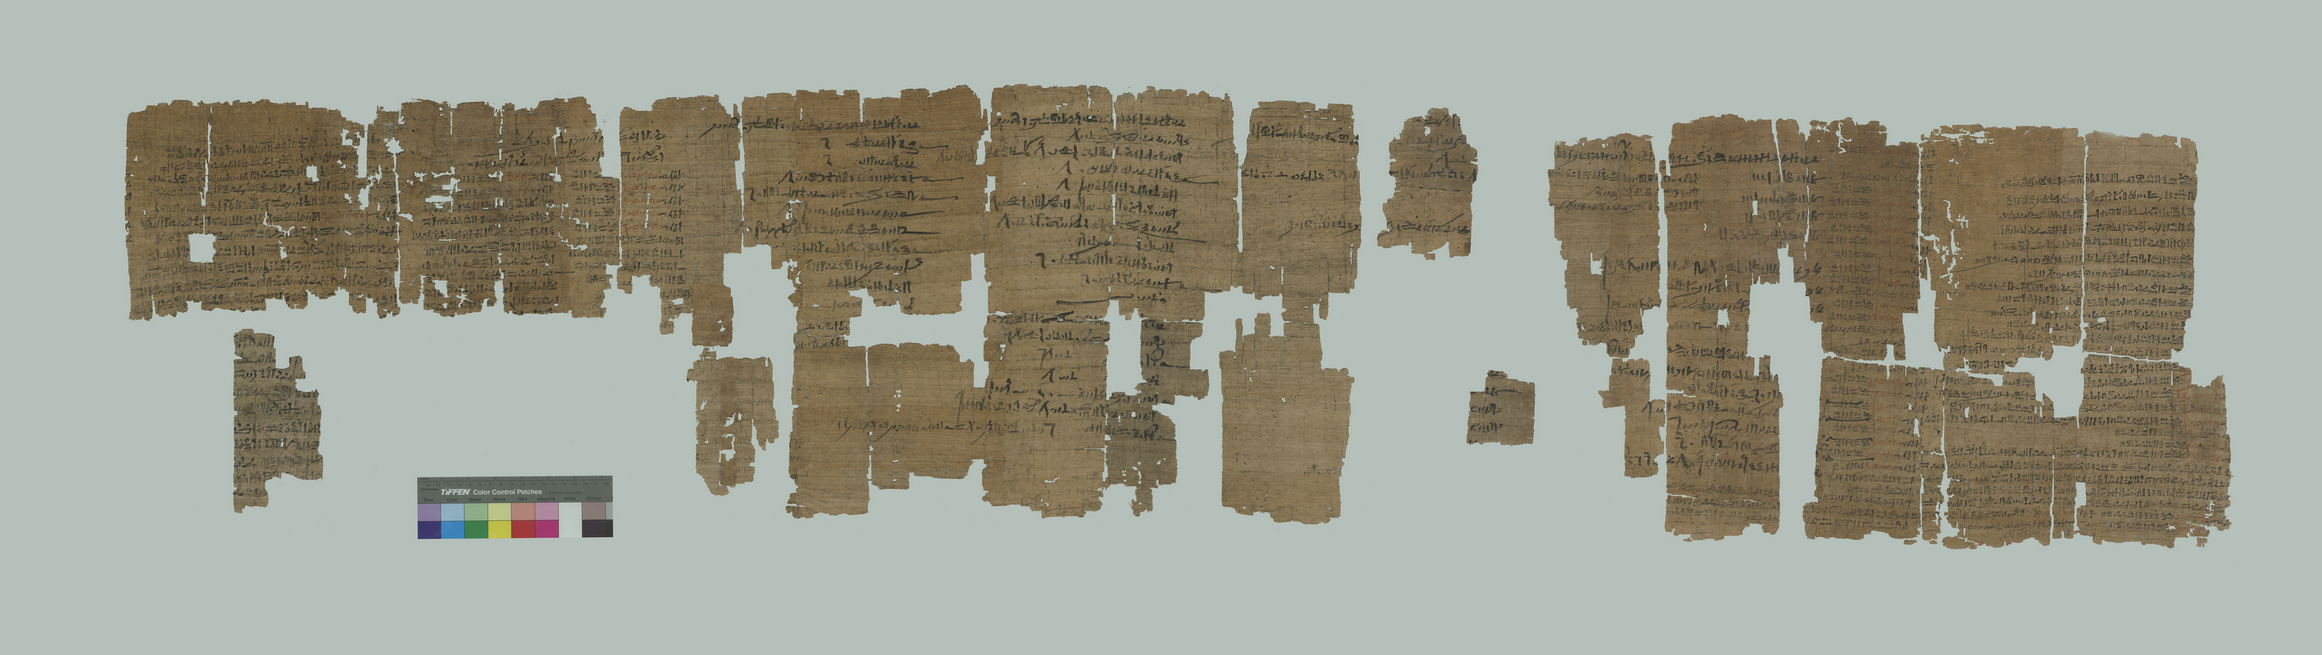
\includegraphics[width=11cm]{papyrus.PNG}
\caption{Example of papyrus fragments from the Deir el-Medina corpus.}
\label{papyrus}
\end{figure}

The process of reassembling fragments into larger manuscripts is very time consuming and far from trivial; it takes a lot of efforts from experts to solve these "jigsaw puzzles", especially with so many small fragments to consider.

\section{Goal of the thesis}

The goal of the present thesis is to use machine learning techniques such as deep neural networks to help egyptologists in the task of papyrus reconstitution, by developing algorithms to detect potentially linked fragments (i.e. originating from the same papyrus) and ease the reconstitution progress.\newline
This piece of work will mainly revolve around the use of siamese neural networks using convolutional architectures (CNNs) to compare papyrus fragments and tell whether they come from the same original papyrus or not.\newline

\newpage


\chapter{Methods}

\section{Introduction to Siamese Networks}

A Siamese neural network (sometimes called twin neural network) is an artificial neural network containing two or more identical subnetwork components that share their weights (hence the name "siamese"). This kind of neural network, first introduced by Bromley et al. in 1994 \cite{bromley94} to tackle the task of automatic signature verification, is specifically designed for tasks involving (dis)similarity.\newline

\begin{figure}[H]
\centering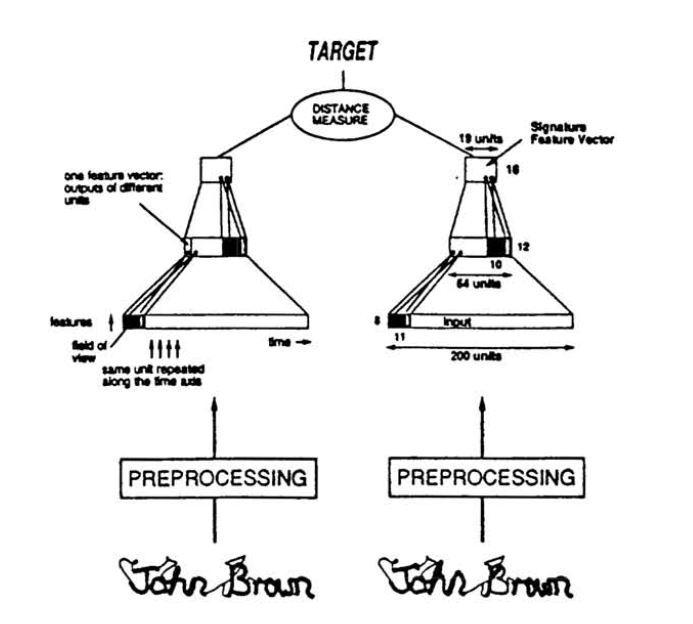
\includegraphics[width=11cm]{siamese94.PNG}
\caption{First siamese neural network architecture, proposed by Bromley et al. in 1994.}
\label{papyrus}
\end{figure}

A typical siamese networks consists in two identical branches (the \emph{twin networks}), each taking an input, that are later combined to compute a \emph{similarity measure} (e.g. a distance metric such as the Euclidean distance) quantifying the similarity between the two branches' end vectors. This similarity measure can be directly outputted, or further used by extending the network (e.g. to perform classification).\newline
It is important that not only the architecture of the twin networks is identical, but the weights have to be shared among them as well. The weight-sharing guarantees that two very similar inputs can not be  mapped  by  their  respective  twin  to  very different points in the feature space, because each twin computes the exact same function.\newline

Technically speaking, the twin networks can consist in any kind of neural network architecture, adapted to any kind of input data (fully-connected for numerical data, convolutional for images, LSTM for sequential data,...), though convolutional networks are often preferred, due to the fact that most applications of siamese networks involve image similarity. The twin networks' purpose is essentially to transform the input data they receive into a feature vector that be conveniently used to compute a similarity measure between the two inputs of the siamese network.\newline 

In the context of the present thesis, where the inputs will be images, siamese networks using convolutional neural networks (CNNs) are the architecture of choice. A simplified representation is given in figure \ref{siam}.


\begin{figure}[H]
\centering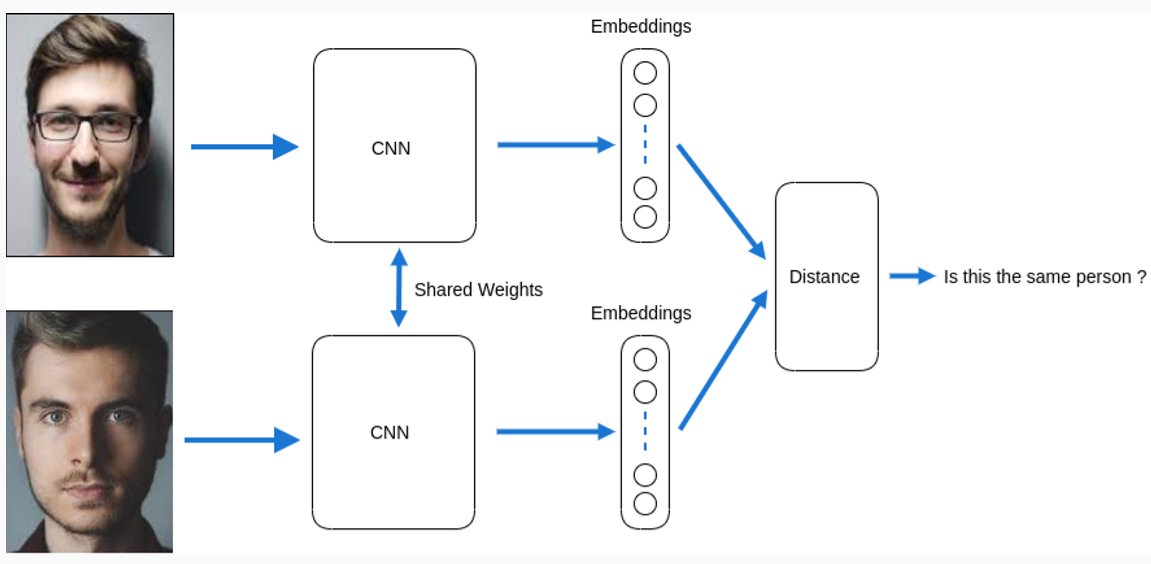
\includegraphics[width=11cm]{siam.PNG}
\caption{Simplified representation of a siamese neural network using a CNN.}
\label{siam}
\end{figure}

In such an architecture, the convolutional part of the siamese network is used to get embeddings (called \emph{output feature maps}) of the input images that capture fine-grained information about them. The embeddings are then used to compute a similarity measure. A simple and commonly used similarity measure is the Euclidean distance (also called $L^2$ norm).\newline
Given two vectors $(x,y) \in \mathbb{R}^p \times \mathbb{R}^p$, the Euclidean distance between them is defined as:
$$d(x,y) = ||x - y||_{2} = \sqrt{\sum_{i = 1}^{p} (x_i - y_i)^2}$$

\section{Architectures}
\label{sec:arch}

Convolutional-based siamese neural networks can be broken down in two main components: the CNN architecture, which is responsible for the embedding of the input images; and the similarity measure, which determines the final output of the network. An optional third component can be used after the similarity measure, for instance to perform classification.\newline

The choice of the CNN architecture will essentially determine the nature of the information encapsulated in the embedding of the input images; not only the depth of the network matters, but also the number and size of the convolutional kernels. These hyperparameters define the receptive field of the network and the number of features it will extract from the images.\newline
In the context of papyrus fragment matching, it may be interesting to investigate the impact of the CNN architecture and determine whether or not a deeper, more complex convolutional architecture is useful to the task.\newline

For that reason, experiments will be conducted on a few convolutional architectures: first, the well-known ResNet architecture (with its ResNet50 variant - 50 layers); then, the Papy-S-Net architecture (or rather, its convolutional part) proposed by Pironne et al. \cite{pir19}; finally, a novel architecture developed in the context of the present thesis, named HieraNet (as we are dealing with hieratic papyri).


\subsection{ResNet50}
\label{subsec:resnet}

The ResNets (\emph{Residual Networks}) were introduced by Kaiming He et al. \cite{res15} as a novel type of very deep architecture that can be efficiently trained using \emph{residual learning blocks} implementing shortcut connections to mitigate the issue of vanishing gradients arising with deep networks.\newline


%Explication resnet avec skip connections


Deep residual networks have been shown to be particularly good at many computer vision tasks; they are therefore intesting to consider for the present task.\newline
The ResNet50 variant is a 50-layers deep convolutional architecture (figure \ref{resnet50}) with over 23 million parameters. It achieved a 20.74\% top-1 validation error (5.25\% top-5) on the ImageNet classification task, and offers the advantages of very deep architectures while being reasonably fast to train.\newline

In order to speed-up the training, as ResNet50 is a quite large network, transfert learning is used. This interesting approach consists in initializing the weights of ResNet50 with weights that were obtained by previously training it extensively on the ImageNet dataset. Using the "knowledge" obtained from the ImageNet dataset, it is possible to improve the learning process for the task of papyrus matching.\newline

\begin{figure}[H]
\centering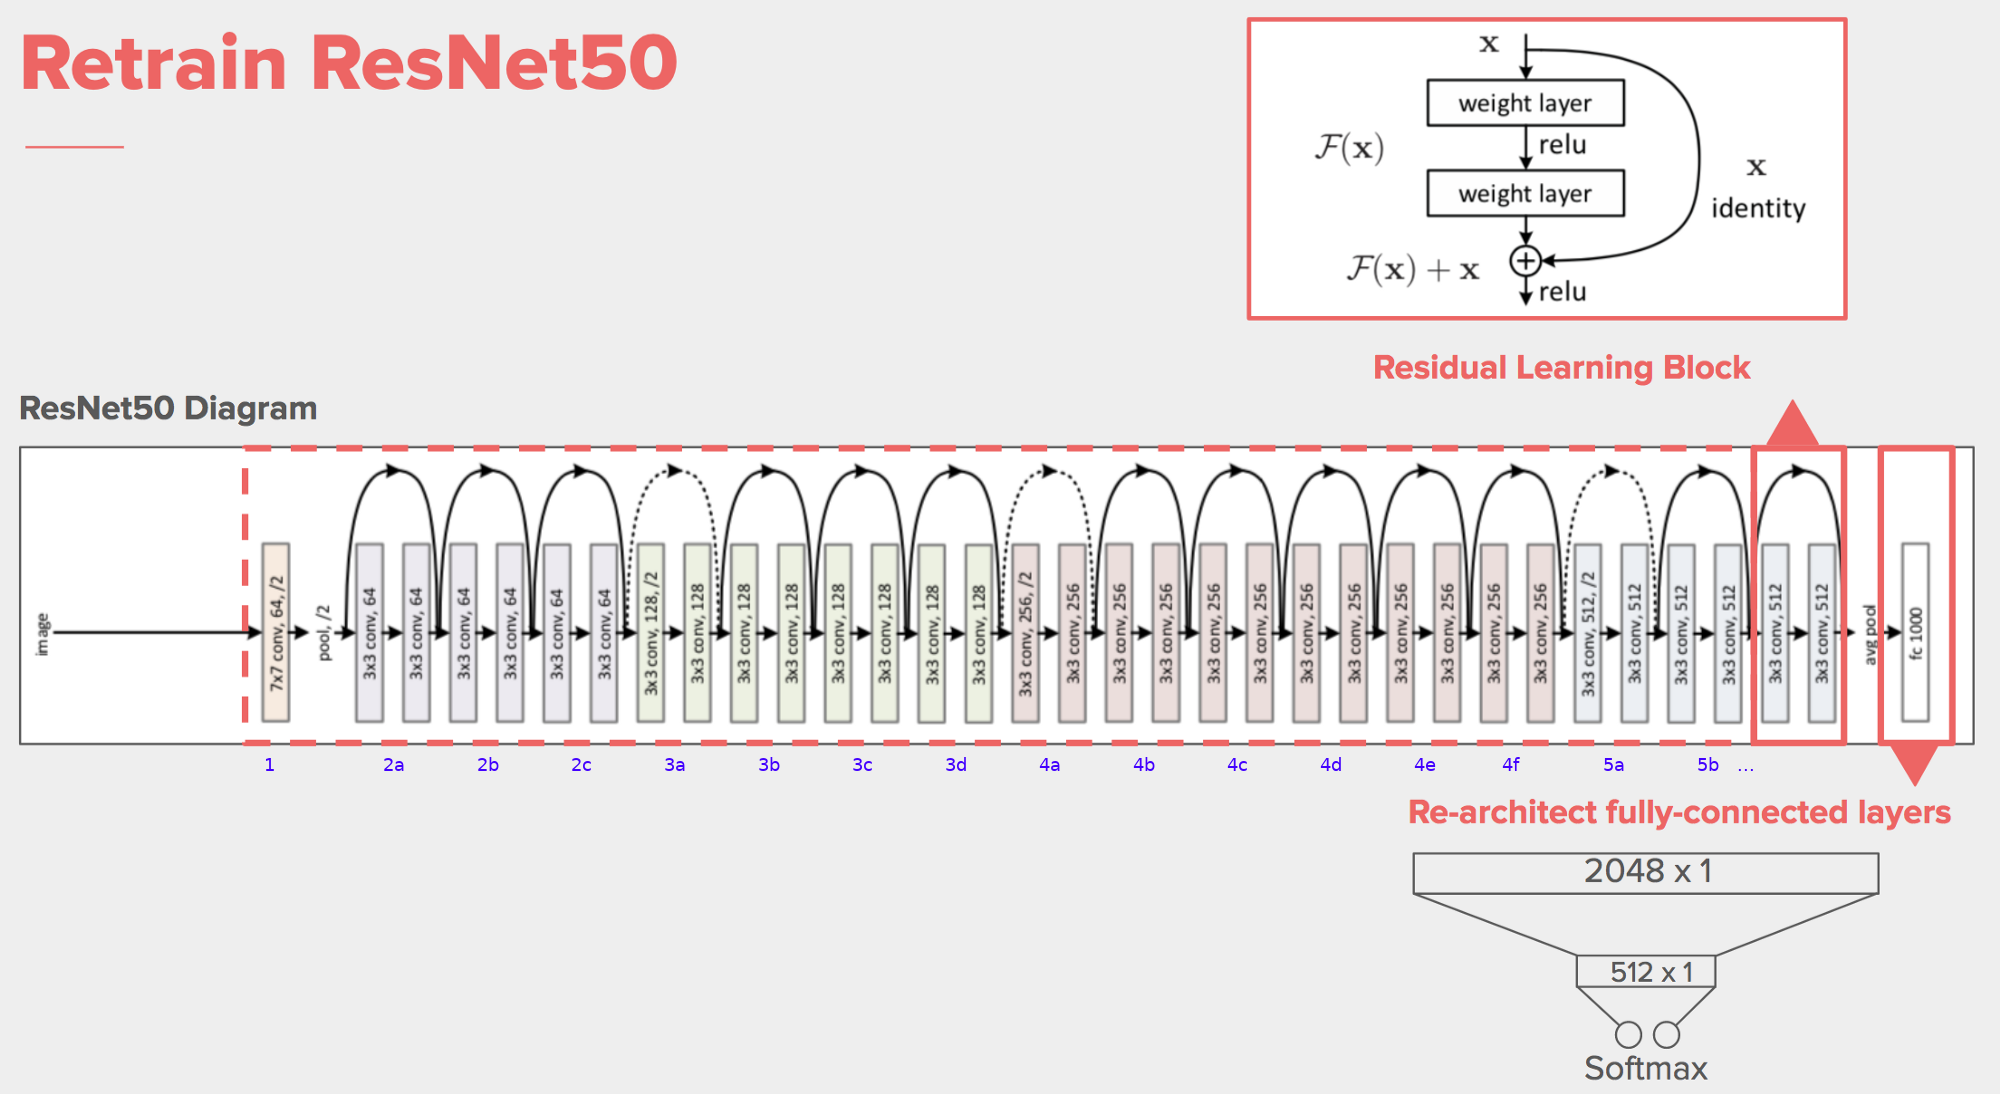
\includegraphics[width=13cm]{resnet50.png}
\caption{The ResNet50 architecture.}
\label{resnet50}
\end{figure}

Using a very deep convolutional architecture, sure as ResNet50, allows to capture very "deep" visual information about the input images. Although in the current state of the art, researchers still fail to completely understand the information captured by CNNs (what they "see"), it is known that deep networks learn particularly complex image patterns, that can be related to shapes, but also textures, for instance. Since papyrus scrolls are made from fibers of the papyrus plant, their texture and the structure of these fibers can be useful information to consider (and in practice, it is indeed considered by scholars). A deep convolutional network might capture this kind of information, although the resolution of the images needs to be quite high in order to clearly see the fibers.\newline

In this thesis, several siamese architectures using ResNet50 are considered, and will now be detailed.\newline

A first variant, labelled \emph{ResNet50-Base}, consists in ResNet50 (with average pooling) followed by a simple euclidean distance (i.e. a layer computing the $L^2$ norm between the two output feature maps) and a softmax. This variant therefore only uses the convolutional part as an encoder for the images, and directly computes the euclidean distance (i.e. a simple scalar) between them before classifying using this distance. As such, most of the information from the convolutional part is "discarded" for the classification.

\begin{figure}[H]
\centering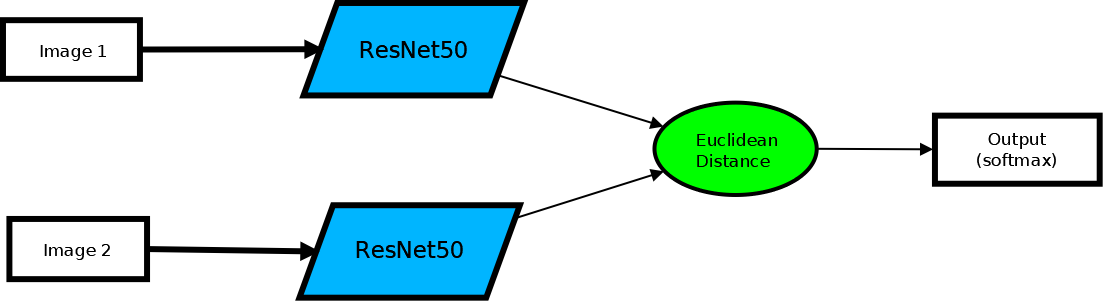
\includegraphics[width=13cm]{diaresbase.png}
\caption{The ResNet50-Base architecture.}
\label{resnet50base}
\end{figure}

The \emph{ResNet50-Full} variant, inspired by the Papy-S-Net architecture (section \ref{subsec:papy}), is quite different as the output feature maps of the convolutional part (again, ResNet50 with average pooling) are flattened, then merged using the absolute difference ($|x-y|$), followed by two fully-connected layers with 512 units each. Here, the information from the convolutional part is retained until the classification.

\begin{figure}[H]
\centering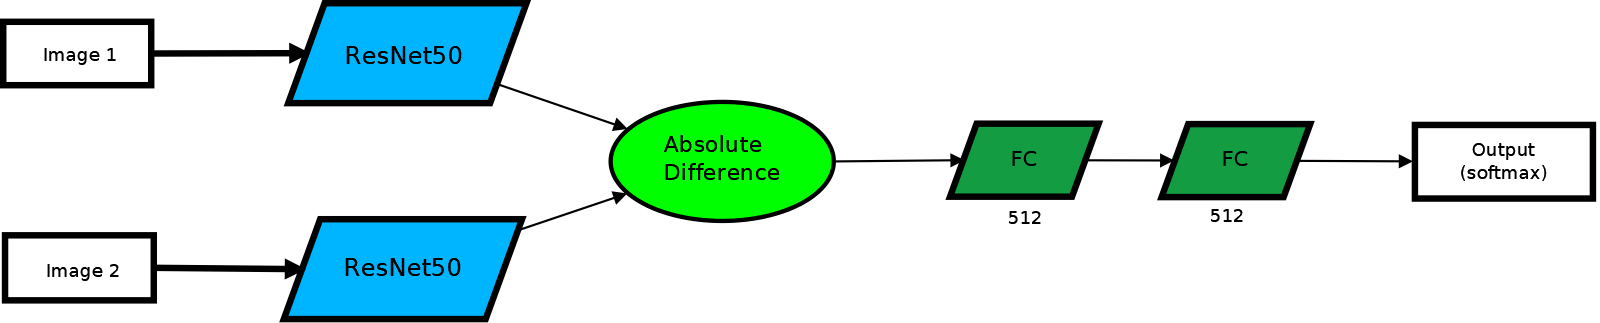
\includegraphics[width=13cm]{diaresfull.png}
\caption{The ResNet50-Full architecture.}
\label{resnet50full}
\end{figure}

\subsection{Xception}\label{subsec:xception}

Xception (short for \emph{Extreme Inception}) is a deep convolutional architecture introduced by Chollet \cite{cho17} in 2017 as an improvement of the InceptionV3 network, taking its principles to an extreme.\newline

The main hypothesis of the Inception and Xception architectures is that for images, cross-channel correlations and spatial correlations are sufficiently decoupled that it is preferable not to map them jointly. In practice, this means that while in a traditional CNNs the convolutional layers seek out correlations across both space (the pixels) and depth (the channels), in Inception and Xception space and depth are considered seperately.\newline

In the case of Xception, so-called \emph{depthwise separable convolutions} are used; first, the spatial correlations of each channel are mapped separately, and then a 1x1 depthwise convolution is used to capture cross-channel correlations (figure \ref{xception_module}.)\newline

\begin{figure}[H]
\centering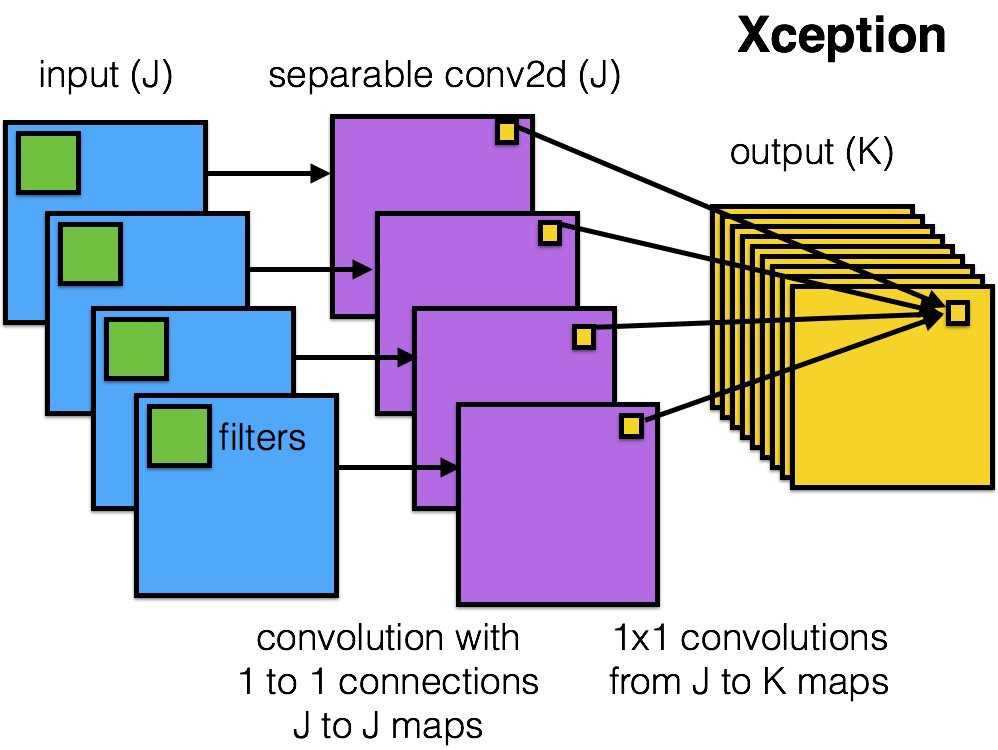
\includegraphics[width=8.5cm]{xception_module.jpg}
\caption{Depthwise separable convolution module, as used in the Xception network.}
\label{xception_module}
\end{figure}

Similarly to ResNet50, two siamese architectures using Xception are considered, with the same approach:\newline

The first variant, called \emph{Xception-Base}, consists in Xception (with average pooling) followed by a simple euclidean distance (i.e. a layer computing the $L^2$ norm between the two output feature maps) and a softmax. As with ResNet50-Base, this variant only uses the convolutional part as an encoder for the images, and directly computes the euclidean distance (i.e. a simple scalar) between them before classifying using this distance. As such, most of the information from the convolutional part is "discarded" for the classification.

\begin{figure}[H]
\centering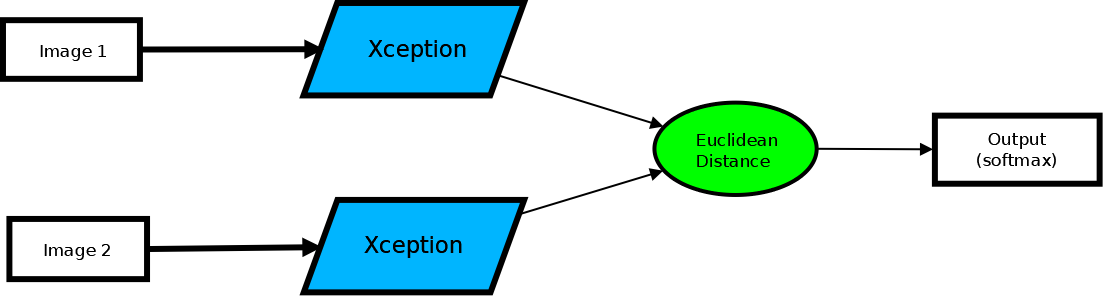
\includegraphics[width=13cm]{diaxcepbase.png}
\caption{The Xception-Base architecture.}
\label{xcepbase}
\end{figure}

The second variant, \emph{Xception-Full}, is similar to \emph{ResNet50-Full}, and makes full use of the Xception architecture by taking the absolute difference of the output feature maps and passing it through a two-layers fully connected network.

\begin{figure}[H]
\centering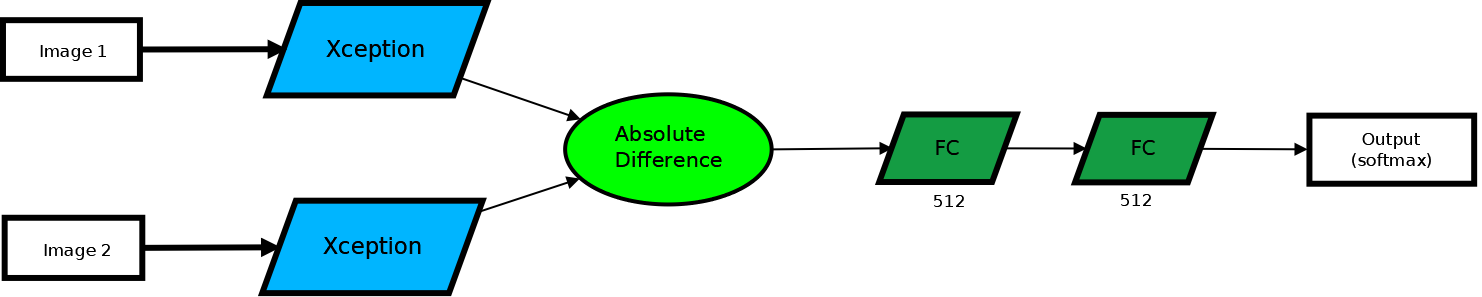
\includegraphics[width=13cm]{diaxcepfull.png}
\caption{The Xception-Full architecture.}
\label{xcepfull}
\end{figure}


\subsection{Papy-S-Net}\label{subsec:papy}

Papy-S-Net (\emph{Papyrus-Siamese-Network}) is a siamese neural network introduced in 2019 by Pirrone et al. \cite{pir19} to tackle a task which is very similar to the one addressed in the present thesis. Their paper focused on the matching of papyrus fragments coming from Egyptian mummy cartonnages, the main difference with the present work being that they considered a multilingual corpus (Greek, Latin, Coptic, Arabic and Hieratic) from the hellenistic period.\newline

Their Papy-S-Net architecture uses a convolutional neural network consisting in three (CONV + MAXPOOLING) blocks, for a total of six convolutional layers which is considerably smaller than ResNet50. For the similarity measure, the absolute difference between the two image embeddings, follewed by two fully connected layers, are used instead of the Euclidean distance. In essence, this means that Papy-S-Net focuses less on the image embeddings, and more on learning how to compute a similarity measure using those embeddings. It is quite different from usual convolutional siamese networks were the similarity measure is often a simple Euclidean distance.

\begin{figure}[H]
\centering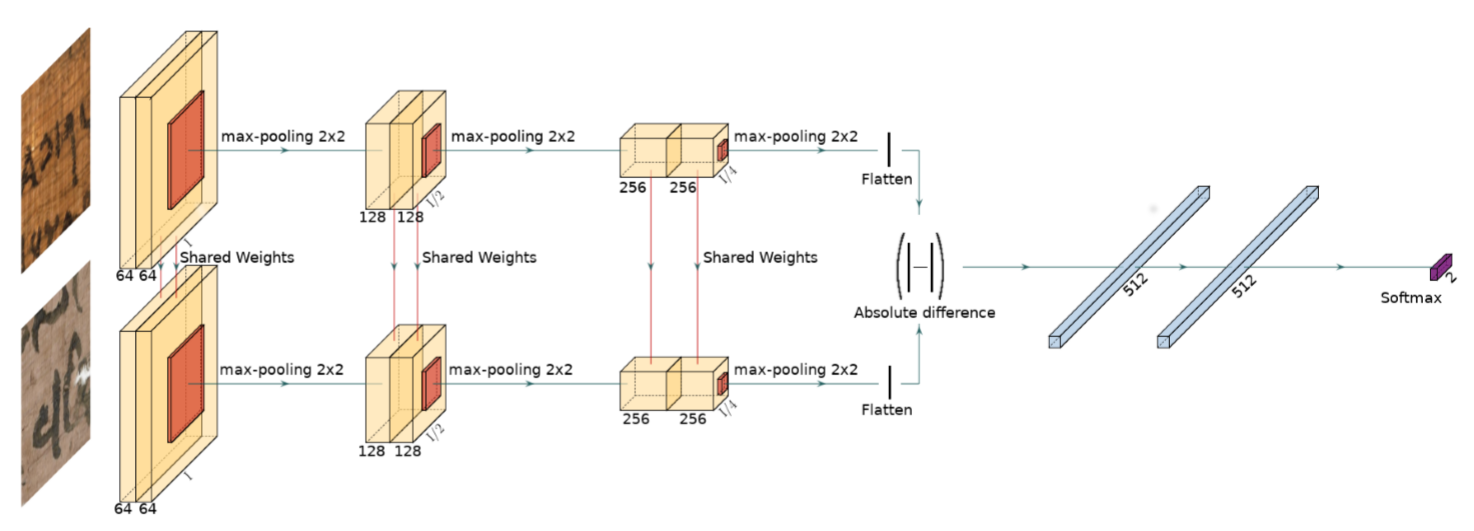
\includegraphics[width=15cm]{papysnet.PNG}
\caption{The Papy-S-Net architecture. (Pirrone et al. '19)}
\label{papysnet}
\end{figure}

\section{Transfer learning}\label{sec:transfert}

Transfer learning is a machine learning technique where a model developed for a task A is reused as the starting point for a model on a second task B, with the goal of speeding up the training process and potentially improving the results. This technique is particularly interesting when the amount of data for task B is lower than for task A; in that case, being able to transfer some "knowledge" from the first task to the other to compensate for the lack of data is interesting.\newline
In the case of papyrus matching, the amount of data available is quite scarce (no large, "standard" dataset exists) and very few models have been developed to tackle this relatively niche task. On the other hand, image classification is a well studied problem with many large datasets and models (among which ResNet50 and Xception) already developed, with impressive results. Since the task of papyrus fragment matching also involves images, transfert learning could potentially be applied successfully.\newline

ImageNet is a vast image dataset consisting of more than 14 million images in 21,841 classes. For years, it has been one of the standard benchmarks to assess the performances of neural networks on the task of image classification, and many models have been developed to push back the state-of-the-art performances on ImageNet. But training neural networks on such a large dataset takes an important  amount of time and computational resources. Therefore, it is difficult to train all models on it, but transfer learning can be (and is) used to still take advantage of the extensive "knowledge" that can be gained from this extensive image dataset.\newline
In fact, most deep learning libraries nowadays propose several architectures (ResNet, Inception, Xception,...) that have been trained on ImageNet, with weights resulting from this training and ready to be fine-tuned on a new task.\newline
In the experiments, the ResNet50 and Xception architectures presented in the previous sections will be used both with random weight initialization and with weights pre-trained on ImageNet, in a tentative to apply transfer learning to the task of papyrus matching.\newline


\chapter{Dataset}

\section{Introduction: provided data \& requirements}

The more than 10,000 papyrus fragments in the Museo Egizio collection are not yet documented in the museum's existing database; their restoration and digitization are still a work in progress. Therefore, the quantity of data available gradually increased throughout the course of this thesis.\newline

The papyrus fragments were directly provided by Mr. Stéphane Polis (University of Liège) and his team in the form of 400dpi scans of papyrus fragments of various sizes, along with larger, already reconstructed papyri. Figure \ref{imageex} presents two of the images provided by the Crossing Boundaries team (these can be considered medium-sized). It is important to note that the digitization procedure can differ from one image to another (e.g. a colour reference chart may or may not be present, the background colour may differ,...).

\begin{figure}[h!]
\centering
  \begin{subfigure}{7cm}
    \centering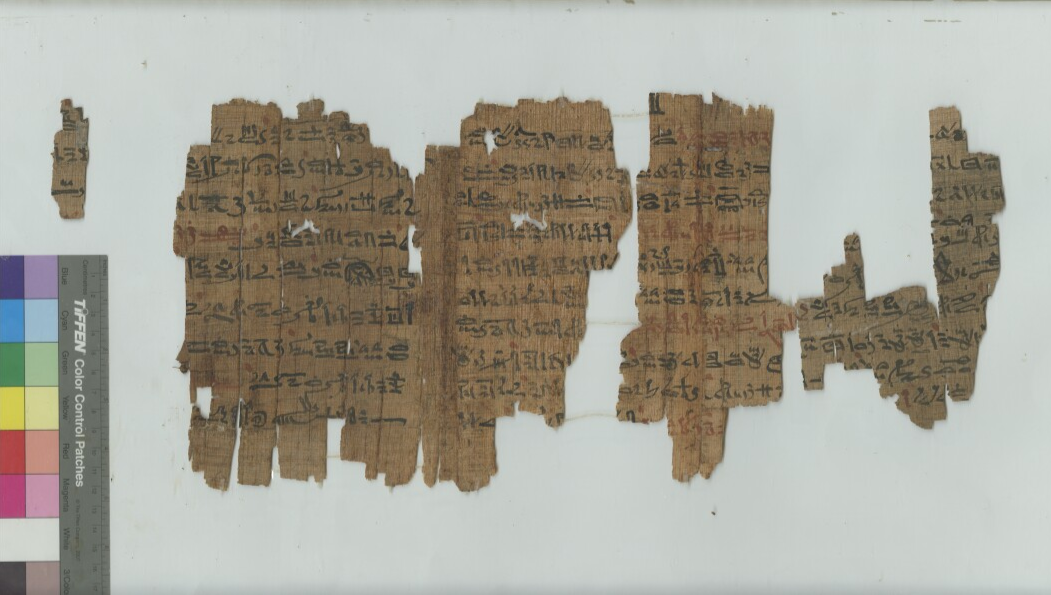
\includegraphics[width=6cm]{papy.PNG}
  \end{subfigure}
  \begin{subfigure}{7cm}
    \centering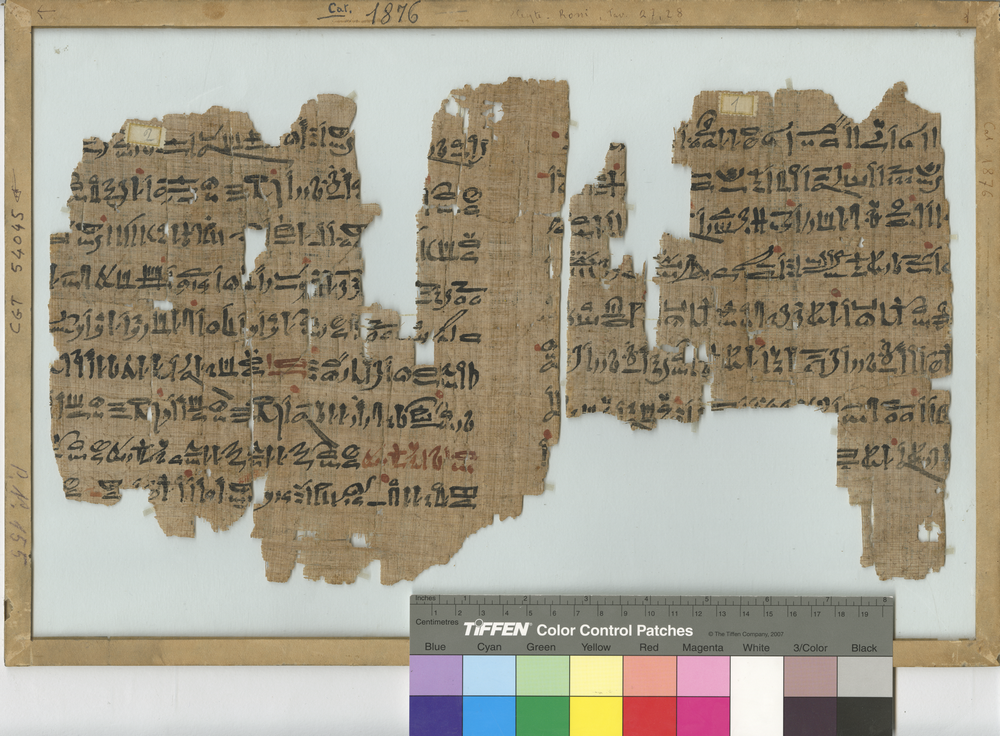
\includegraphics[width=6cm]{papy2.png}
  \end{subfigure}
\caption{Example of images provided by the Crossing Boundaries team. Notice the wooden frame in the second scan.}
\label{imageex}
\end{figure}

Furthermore, the papyri themselves come in all shapes, sizes, colors, and preservation state. Depending on various factors, such as the storage conditions, the visual aspect of the papyri can be altered: while it can sometimes be useful to match fragments, it can also be misleading as different fragments from the same papyri may have been stored in different conditions, resulting in very different visual aspects.\newline

Naturally, these high-resolution scans can not be used \emph{as is} to train models. As explained in section \ref{sec:arch}, the models' inputs are pairs of fragment images. To create an exploitable dataset, it is therefore necessary to extract  (fake) fragments from these high-resolution images to generate \emph{ground truth}, and training data.\newline

For convenience, and as will be seen in the next section, because of the interesting tools provided, all the data has been stored on the \emph{Cytomine} platform of the University of Liège.

\section{Cytomine platform}

The Cytomine open-source software\footnote{https://uliege.cytomine.org/} is an application which fosters collaborative analysis of very large images and allows the semi-automatic processing of large image collections via machine learning algorithms. Although the main usage of Cytomine is medical research, the functionalities provided by the software can be used for any task involving large images.\newline

In particular, Cytomine uses an annotation system that allows users to draw and save "regions of interest" inside the images, and associate values (text description, tags, properties,...) to them. This feature was particularly interesting in the context of the present thesis as it offered a convenient way to build a working dataset (figure \ref{annotation}).

\begin{figure}[h!]
\centering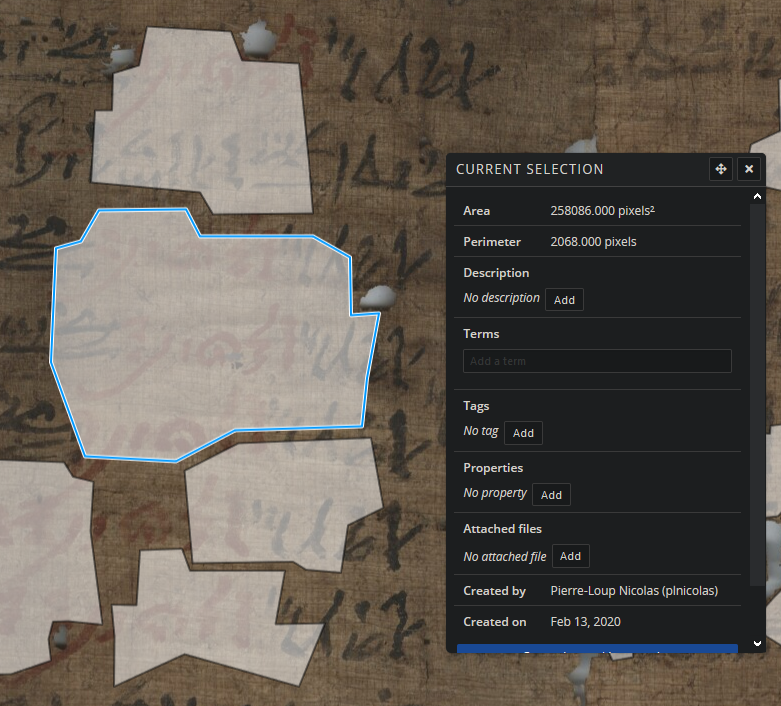
\includegraphics[width=10cm]{annotation.PNG}
\caption{Example of annotations made with the Cytomine web interface.}
\label{annotation}
\end{figure}

The Cytomine web interface allows the user to manually create annotations of various shapes using different tools (freehand, circle, polygon,...), that can subsequently be retrieved in the form of images, either as plain, rectangular crops (thus discarding the original shape of the annotations if not rectangular) or as "alphamasks", i.e. using a transparency mask to preserve the original shape of the annotations (figure \ref{compcrop}).

\begin{figure}[h!]
\centering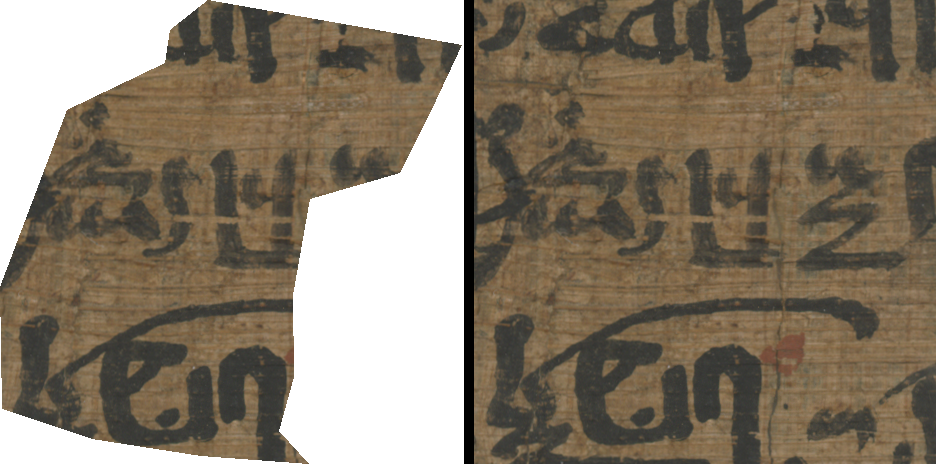
\includegraphics[width=10cm]{compcrop.PNG}
\caption{Comparison between the same annotation extracted either as an alphamask (left) or a crop (right).}
\label{compcrop}
\end{figure}

In the context of papyrus fragment matching, one could think that creating realistic shapes mirroring real fragments might be interesting to train the models; with the Cytomine software, testing such an hypothesis is quite easy (although time-consuming), and this will be investigated in the first experiment, presented in section \ref{experimentbound}.


\section{Creation of the dataset}
\label{sec:data}

During the course of this master thesis, approximately 100 "large", already (partially) reconstructed papyri were sent by the Crossing Boundaries team, along with thousands of small fragments. For each papyrus/fragment, both the recto and the verso were provided. All the images were uploaded on the Cytomine platform of the university of Liège for storage.\newline

From there, the annotation system of the Cytomine platform was used to manually create fake papyrus fragments using the larger papyri, in order to create ground truth.\newline
Initially, these fake fragments ($\approx 1800$ of them) were created with realistic shapes, with the hypothesis that the shape of the fragments might be useful to train the models. However, and as will be seen in the first experiment (section \ref{experimentbound}), the impact is negligible. It is in fact quite easy to understand why: as explained before, for most papyri some of the fragments were lost to time, and furthermore the remaining fragments suffered from several depredations (insects,...), meaning that the shapes of fragments belonging together will, perhaps counter-intuitively, hardly match in practice.\newline
Therefore, and because the task of creating "realistic" fake fragments was tedious and time-consuming, the remaining fake fragments were created as simple, rectangular shapes.\newline

In total, \xfrag fake fragments were created in the form of Cytomine annotations on the large papyri's images. Using the Cytomine API, these annotations can be easily retrieved from the server as images using a simple Python script generating in parallel a CSV file listing, for each image (fake fragment), the papyrus it is coming from. This is the dataset that will be used in all of the experiments.\newline

Since siamese neural networks take image pairs as input, the "fake fragment dataset" is not usable as-is; it is used to generate fragment pairs.\newline
First, in order to avoid any bias between the training and test data, the fake fragments are split into two sets, according to their source papyrus: the training fragments set $S_{train}$, and the test fragments set $S_{test}$. 75\% of the papyri are used for $S_{train}$, and the remaining 25\% for $S_{test}$.\newline

For both $S_{train}$ and $S_{test}$, \emph{positive pairs} (the two fragments come from the same papyrus) and \emph{negative pairs} (the two fragments do not come from the same papyrus) are generated for each papyrus in the set, using a very simple procedure which simply consists in sampling fragments from the dataset and combining them (duplicate pairs are discarded).\newline
This simple procedure makes it possible to generate an arbitrary large number of positive and negative pairs. Indeed, if the dataset consists in $k$ distinct papyri, with $n$ fake fragments each, there are $k \times \overline{C}_{2}^{n} = k \times \frac{n \times (n+1)}{2}$ distinct positive pairs, and $k \times [n \times ((k - 1) \times n)]$ distinct negative pairs. Thus, assuming a relatively small dataset of $n = 50$ fake fragments per papyrus, with $k = 20$ papyri, 25500 positive and 950000 negative pairs are already possible.\newline
However, the number $k$ of different papyri should be as large as possible, to ensure sufficient diversity in the dataset; sampling a very large number of pairs from only a few papyri would undoubtedly lead to models that fail to generalize properly to never-seen papyri.\newline


\chapter{Methodology}

\section{Test protocol \& evaluation metrics}

In order to conduct the experiments, as presented in section \ref{sec:arch}, the fake fragments dataset consisting in \xfrag fake fragments from \xpapy distinct papyri is used to generate a total of TBD training pairs and TBD test pairs, the former being generated from 75\% of the papyri and the latter with the remaining 25\%.\newline

Each model is trained for 40 epochs with a batch size of 16, using the Adam optimizer with default parameters and categorical cross-entropy as the loss function. The input images' size and the learning rate vary depending on the network; these parameters are given in the section relative to each experiment. Furthermore, unless noted otherwise, data augmentation is used, in the form of random horizontal and vertical flips (probability of 0.5 for both). The impact of this data augmentation and other data augmentation methods will be investigated in one of the experiments.\newline

The evaluation metrics for the different models are the train and test accuracy, but also (and perhaps more importantly) the precision and recall, two metrics originating from the field of information retrieval that are particularly relevant in the context of the task of papyrus fragment matching.\newline
Precision is the ratio of correctly predicted positive observations to the total predicted positive observations, and is computed\footnote{TP = True Positives, TN = True Negatives, FP = False Positives, FN = False Negatives.} as
$$p = \frac{TP}{TP + FP}$$
The precision essentially represents the confidence we can put in the model when it predicts a case as positive. Recall (also known as sensitivity or true positive rate) is the proportion of positive observations that are detected among all positive observations, and is computed as
$$r = \frac{TP}{TP + FN}$$
The recall is a measure of how well the model recognizes positive observations.\newline
Ideally, precision and recall should both be as high as possible, but usually there is a trade-off between them.\newline

From these two measures, we can also define the F1-score, which is computed as a weighted average of precision and recall:
$$F1 = \frac{2 \times Precision \times Recall}{Precision + Recall}$$

These metrics are often presented in the form of ROC curves and precision-recall curves.\newline

\subsection{ROC Curves}

ROC (\emph{Receiver Operating Characteristic}) curves plot the recall as a function of the \emph{1-sensitivity}, also called false positive rate \footnote{Defined as $\frac{FP}{FP + TN}$.} with varying confidence thresholds. It illustrates the predicting ability of a binary classifier as its confidence thresholds varies.\newline
In practice, the predictions of the classifier are sorted from the most confident to the least confident, and the confidence threshold is varied. Each value of the threshold yields a different confusion matrix from which the recall and 1-sensitivity can be computed, corresponding to a point of the curve. Figure \ref{ROCexemple} gives an exemple of ROC curve for some binary classifier.

\begin{figure}[h!]
\centering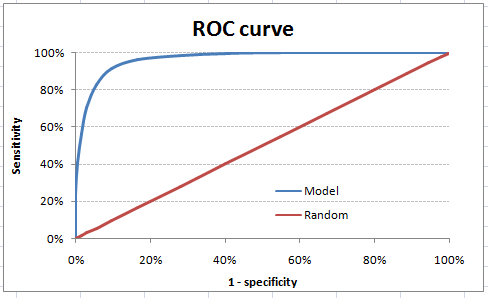
\includegraphics[width=10cm]{ROCexemple.png}
\caption{Example of ROC curve of some model (blue) and a random classifier (red).}
\label{ROCexemple}
\end{figure}

Intuitively, at the point (0,0), the classifier always categorize an observation as a negative case: there is no false positive, but there is no true positive either. At (1,1), the classifier always categorize an observation as a positive: there is no true negative, but no false negative either. Thus a random classifier would give a flat ROC curve passing through the points (0,0) and (1,1).\newline
On the other hand, a perfect classifier would yield a ROC curve passing through the point (0,1), i.e. no false positive and no false negative. A good model will thus be characterized by a ROC curve tending towards the point (0,1). For that reason, it is often convenient to summarize the ROC curve by a single value, called the \emph{area under the curve} (AUC); the AUC is equal to 1 for a perfect classifier and to 0.5 for a random one. In general, the higher the AUC, the better the predictions.\newline

\subsection{Precision-Recall Curves}

Similarly, Precision-Recall (PR) curves plot the precision as a function of the recall when varying the confidence threshold. Here, a perfect classifier would pass through the point (1,1), and once again, the area under the curve, called MAP (for \emph{Mean Average Precision}) can be used to summarize it; the higher the MAP, the better the predictions. One thing important to note, however, is that while ROC curves are independent of the ratio between positive and negative observations, PR curves are not; therefore, class imbalance can be an issue when considering Precision-Recall curves.\newline

\section{Visualization techniques}

On top of these metrics, it can be interesting to visualize the predictions of the models. Because the task of papyrus fragment matching involve learning a (dis)similarity/distance measure, it is relatively well-suited for visualization techniques such as hierarchical clustering methods, multidimensional scaling and the t-SNE algorithm. While these methods are not necessarily a mathematically rigorous way of assessing the results, they represent a convenient way to look at them and could provide interesting information.\newline

These visualization techniques only require a distance matrix giving distance measurements between objects; and such a distance matrix can easily be obtained from the neural networks considered in this thesis.\newline
The architectures presented in section \ref{sec:arch} end with a softmax layer, meaning that they output, for each input pair, a vector of two elements: the probability $P_0$ given by the network of the input belonging to class 0 (i.e. "similar pair"), and the probability $P_1$ of the input belonging to class 1 (i.e. "dissimilar pair"), which is of course $1 - P_0$.\newline
The closer $P_0$ is to 1, the more confident the network is about the fragments in the input pair being similar (and belonging to the same original papyrus); conversely, if $P_1$ is close to 1, the network considers that the fragments are dissimilar and do not belong to the same papyrus. Therefore, $P_1$ can be seen as a \emph{distance measure} between the fragments in the input pair, and this value can be used to build a distance matrix for a given set of fragments.\newline

It is thus possible to build a distance matrix directly from a model's prediction for a set of fragment pairs.\newline


\subsection{Hierarchical clustering}

Hierarchical clustering groups similar objects into entities called clusters. The objective is to iteratively define clusters that are distinct from each others, and for which the objects within each cluster are broadly similar to each other.\newline
Several hierarchical clustering strategies exist, using either an agglomerative (bottom-up, i.e. start from clusters containing a single object and aggregate iteratively) or divisive (top-down, i.e. start with all objects belonging to a single cluster and divide it iteratively) approach.

\begin{figure}[h!]
\centering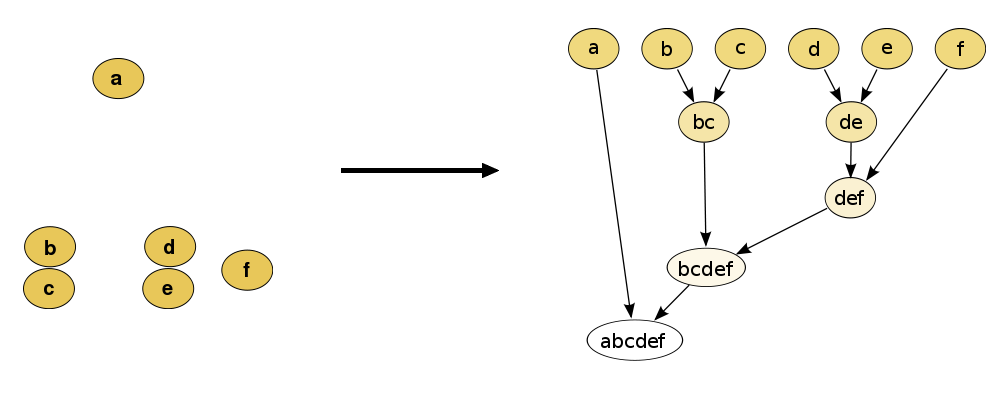
\includegraphics[width=12cm]{hierar.png}
\caption{Illustration of agglomerative hierarchical clustering; raw data on the left, resulting dendrogram on the right.}
\label{ROCexemple}
\end{figure}

Hierarchical clustering has the distinct advantage that any valid measure of distance can be used. Even the observations themselves are not required: all that is used is a matrix of distances.

\chapter{Experiments}

\section{Impact of the fragment boundaries}\label{experimentbound}

The objective of the first experiment is to determine whether considering the exact shape of the fragments is useful to tackle the task, or not. As already mentioned in section \ref{sec:arch}, creating fake fragments of realistic shapes is a very tedious and time consuming process, thus evaluating their usefulness is particularly important. Furthermore, this question has not been addressed by the literature yet, as Pironne et al. (\cite{pir19}) used rectangular crops in their experiments. \newline

In this first experiment, only the Papy-S-Net architecture is considered.\newline
In total, 1812 fake fragments coming from 22 different papyri are used; the 15 biggest papyri yielded around 100 fragments each, while the 7 smaller ones yielded 25 to 60 fragments each, depending on their size. Although 22 papyri is not a very large number, the selection is quite diverse in colors, preservation state, etc.\newline
From these fragments, 104,198 training pairs and 43,613 testing pairs are generated. The image size is 128x128.\newline
For both the crops and the alphamasks, the learning rate is set at 0.0001 for the first 20 epochs, and 0.00001 for the remaining 20 epochs.

\begin{figure}[h!]
\centering
  \begin{subfigure}{8cm}
    \centering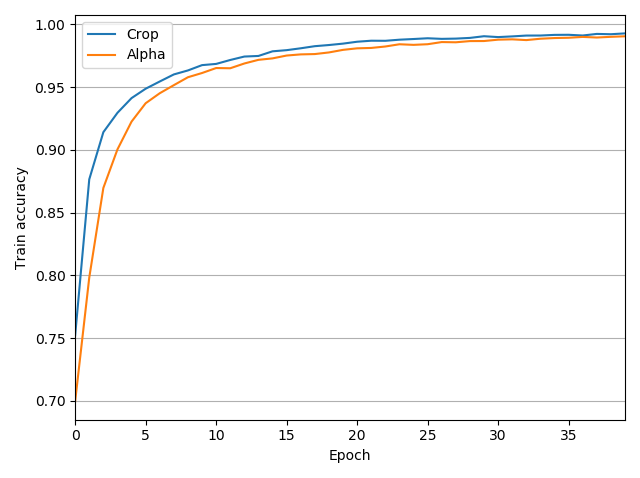
\includegraphics[width=7.5cm]{plot_train_cropalpha.png}
  \end{subfigure}
  \begin{subfigure}{8cm}
    \centering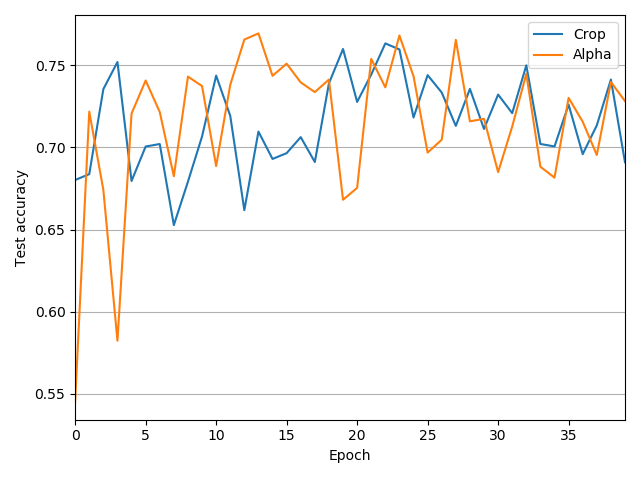
\includegraphics[width=7.5cm]{plot_test_cropalpha.png}
  \end{subfigure}
\caption{Train (left) and test (right) accuracy of the Papy-S-Net architecture when using regular crops or alphamasks.}
\label{alphavscrop}
\end{figure}

Figure \ref{alphavscrop} shows the compared performances of the Papy-S-Net architecture when using crops or alphamasks, while tables \ref{tab:tabpapycrop} and \ref{tab:tabpapyalpha} give the evaluation metrics of both approaches. At first glance, it seems that the impact of the alphamask is quite negligible, as in botch cases the train and test accuracy are very similar. The evaluation metrics confirm this observation, giving a slight advantage to the model using regular crops.\newline

\begin{table}[h!]
\begin{tabular}{l|l|l|l|}
\cline{2-4}
                                             & Precision & Recall & F1-Score \\ \hline
\multicolumn{1}{|l|}{Class 0 (= similar)}    & 0.70      & 0.79   & 0.74     \\ \cline{1-1}
\multicolumn{1}{|l|}{Class 1 (= dissimilar)} & 0.79      & 0.70   & 0.75     \\ \hline
\multicolumn{1}{|l|}{Weighted average}       & 0.75      & 0.74   & 0.74     \\ \hline
\end{tabular}
\caption{Evaluation metrics for Papy-S-Net using crops.}
\label{tab:tabpapycrop}
\end{table}

\begin{table}[h!]
\begin{tabular}{l|l|l|l|}
\cline{2-4}
                                             & Precision & Recall & F1-Score \\ \hline
\multicolumn{1}{|l|}{Class 0 (= similar)}    & 0.76      & 0.72   & 0.47     \\ \cline{1-1}
\multicolumn{1}{|l|}{Class 1 (= dissimilar)} & 0.77      & 0.80   & 0.75     \\ \hline
\multicolumn{1}{|l|}{Weighted average}       & 0.77      & 0.77   & 0.62     \\ \hline
\end{tabular}
\caption{Evaluation metrics for Papy-S-Net using alphamasks.}
\label{tab:tabpapyalpha}
\end{table}


It is clear that in both cases, the network heavily overfits the data, as the train-set accuracy quickly stabilizes at over 95\% while the test-set accuracy oscillates between 70 and 75\%. The overfitting is mainly due to the small amount of data used for this preliminary test (1812 distinct fake fragments vs. \xfrag in the subsequent experiments). As a result, while it can be observed that the alphamasks (i.e. the shapes of the fragments) have a negligible impact, it is necessary to remain cautious as this observation come for a limited amount of data.\newline
But due to time constraints and because simple RGB images are more convenient to work with, the approach of using realistic shapes for the fake fragments is abandoned in the subsequent experiments. As will be seen in the next section, it is possible to obtain interesting results nonetheless.\newline

\section{Preliminary experiments}

A first batch of experiments has been conducted on the first "iteration" of the dataset, consisting in only 1812 fake fragments from 22 distinct papyri (cf. section \ref{experimentbound}); as will be seen, overfitting is a core issue at this stage. These experiments have been conducted again on the second, larger iteration of the dataset, thus these preliminary results are presented here to assess the impact of adding additional data.\newline

In this experiment, four architectures are considered (see section \ref{sec:arch} for details): ResNet50-Base, ResNet50-Full, Xception-Base and Xception-Full. For each of them, two variants are used: the first one uses random weight initialization, while the second one uses weights pre-trained on the ImageNet dataset (cf. section \ref{sec:transfert}). These variants will be respectively called "Random" and "IN".\newline

The input image sizes, initial learning rate and learning rate schedule are given in table \ref{prelimtable}. These parameters are used by both the Random and IN variants of the architectures.

\begin{table}[h!]
\begin{tabular}{l|l|l|l|}
\cline{2-4}
                                    & Image size & Initial LR & LR decay factor                                             \\ \hline
\multicolumn{1}{|l|}{ResNet50-Base} & 224x224    & 0.01                  & x0.2, after 5 epochs without improvement of val. loss \\ \hline
\multicolumn{1}{|l|}{ResNet50-Full} & 224x224    & 0.0001                & x0.1, once, after 20 epochs                                 \\ \hline
\multicolumn{1}{|l|}{Xception-Base} & 224x224    & 0.01                  & x0.2, after 5 epochs without improvement of val. loss \\ \hline
\multicolumn{1}{|l|}{Xception-Full} & 224x224    & 0.0001                & x0.1, once, after 20 epochs                                 \\ \hline
\end{tabular}
\caption{Training parameters for the four architectures in the preliminary experiment.}
\label{prelimtable}
\end{table}

Figure \ref{resnetprelim1} presents the train and test accuracy of the different ResNet50 variants after training for 40 epochs. As in the first experiment with Papy-S-Net, overfitting is a clear issue, which is not surprising. Overall, ResNet50-Base-IN achieves the best test accuracy, at $\approx$ 75\%. The two variants using random weight initialization perform slightly worse.\newline
ResNet50-Full-IN obtains the highest train accuracy, but unsurprisingly given the overall overfitting, the lowest test accuracy, under 60\%.\newline

\begin{figure}[h!]
\centering
  \begin{subfigure}{8cm}
    \centering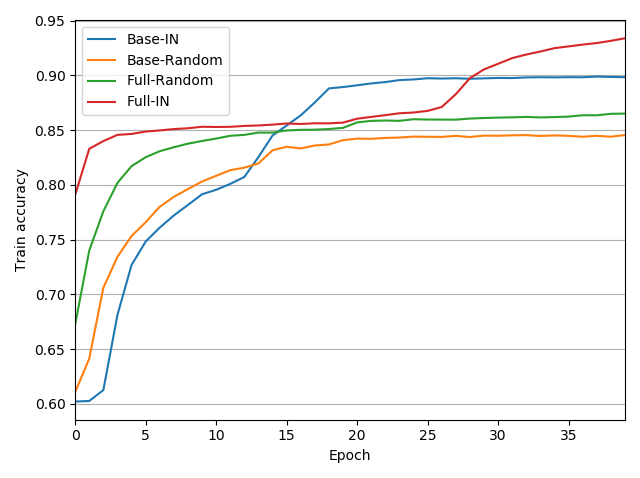
\includegraphics[width=7.5cm]{plot_train_acc_res1.png}
  \end{subfigure}
  \begin{subfigure}{8cm}
    \centering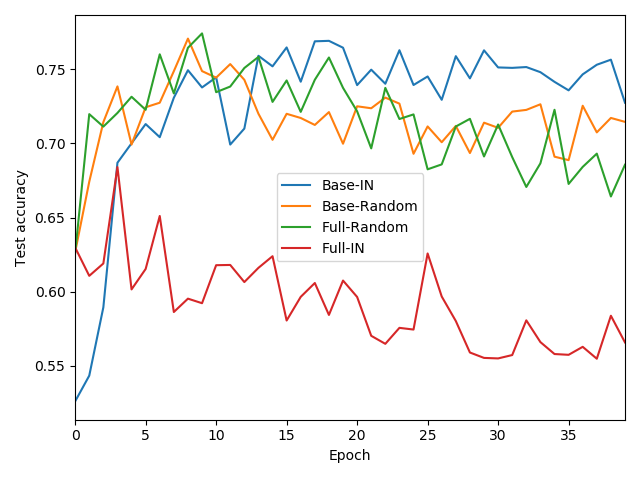
\includegraphics[width=7.5cm]{plot_test_acc_res1.png}
  \end{subfigure}
\caption{Train (left) and test (right) accuracy of the ResNet50 variants.}
\label{resnetprelim1}
\end{figure}

Table \ref{tab:tabresprel1} gives the evaluation metrics for ResNet50-Base-IN, the best performing model. The recall is significantly higher than for Papy-S-Net while the precision remains at 0.88, a notable improvement.

\begin{table}[h!]
\begin{tabular}{l|l|l|l|}
\cline{2-4}
                                             & Precision & Recall & F1-Score \\ \hline
\multicolumn{1}{|l|}{Class 0 (= similar)}    & 0.88      & 0.47   & 0.61     \\ \cline{1-1}
\multicolumn{1}{|l|}{Class 1 (= dissimilar)} & 0.68      & 0.95   & 0.79     \\ \hline
\multicolumn{1}{|l|}{Weighted average}       & 0.77      & 0.73   & 0.71     \\ \hline
\end{tabular}
\caption{Evaluation metrics for ResNet50-Base-IN.}
\label{tab:tabresprel1}
\end{table}

On the other hand, ResNet50-Full-IN yields the worst metrics (table \ref{tab:tabresprel2}). In particular, and quite surprisingly, its recall is extremely low for class 0. In fact, it appears that the network almost always predicts class 1, a tendency that increases as the training goes on and may indicate that the training does not converge.\newline

\begin{table}[h!]
\begin{tabular}{l|l|l|l|}
\cline{2-4}
                                             & Precision & Recall & F1-Score \\ \hline
\multicolumn{1}{|l|}{Class 0 (= similar)}    & 0.72      & 0.08   & 0.14     \\ \cline{1-1}
\multicolumn{1}{|l|}{Class 1 (= dissimilar)} & 0.56      & 0.97   & 0.71     \\ \hline
\multicolumn{1}{|l|}{Weighted average}       & 0.63      & 0.57   & 0.45     \\ \hline
\end{tabular}
\caption{Evaluation metrics for ResNet50-Full-IN.}
\label{tab:tabresprel2}
\end{table}

Similar observations can be made for the Xception networks. Figure \ref{xceptionprelim1} presents the results of the four Xception variants. Here, the best performing models (in terms of test accuracy) are Xception-Base-IN and Xception-Base-Random, at almost 80\%. On the other hand, the Xception-Full variants perform quite poorly.\newline

\begin{figure}[h!]
\centering
  \begin{subfigure}{8cm}
    \centering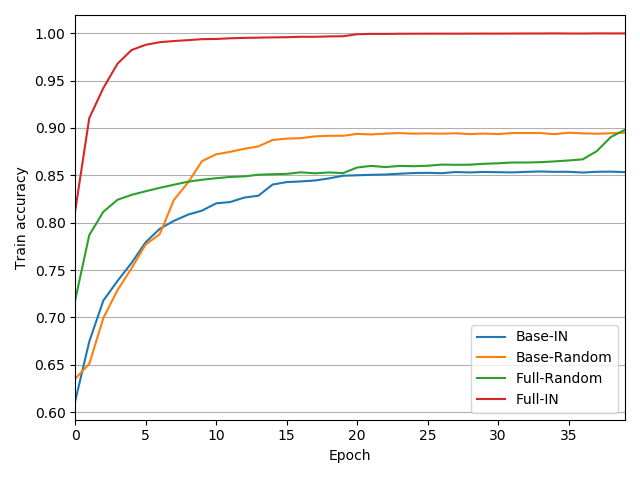
\includegraphics[width=7.5cm]{plot_train_acc_xcep.png}
  \end{subfigure}
  \begin{subfigure}{8cm}
    \centering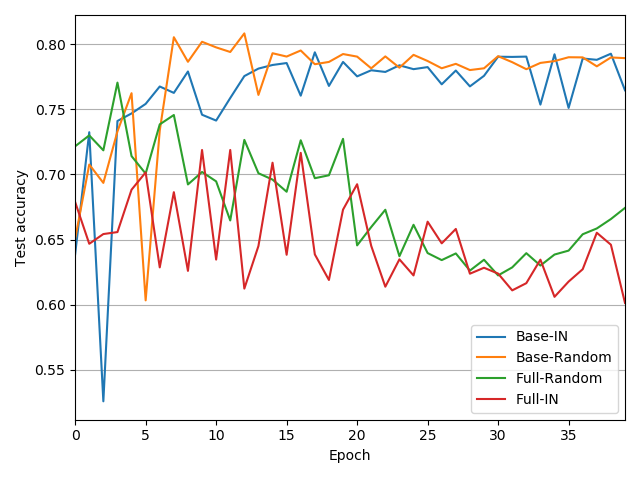
\includegraphics[width=7.5cm]{plot_test_acc_xcep.png}
  \end{subfigure}
\caption{Train (left) and test (right) accuracy of the Xception variants.}
\label{xceptionprelim1}
\end{figure}

Interestingly, the Xception-Base models show a lower tendency to overfit the data, although a quick look at the training and test loss of one of those models is sufficient to see that the issue remains (figure \ref{lossxcepprel}). The subsequent experiments, done on a larger dataset, will focus on reducing the overfitting and improving the generalization capability of the models.

\begin{figure}[H]
\centering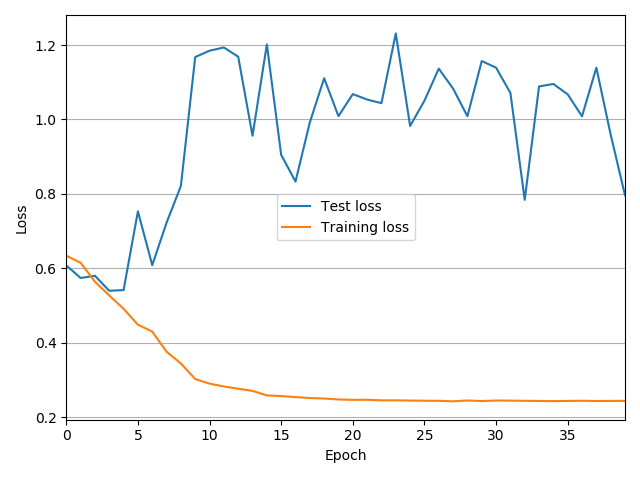
\includegraphics[width=10cm]{plot_loss_xcep_base_random.png}
\caption{Evolution of the training and test loss of Xception-Base-Random during training.}
\label{lossxcepprel}
\end{figure}



Table \ref{tab:tabxcepprel1} gives the evaluation metrics for Xception-Base-Random, the overral best performing Xception model in terms of accuracy. The recall for similar pairs is a lot higher than for the ResNet50 variants while the precision stays roughly the same, which makes Xception-Base-Random the best performing model in this first experiment. Conversely, and as with the ResNet50 variants, Xception-Full-IN gives the lowest metrics, with in particular a recall of 0.15 for matching pairs.

\begin{table}[h!]
\begin{tabular}{l|l|l|l|}
\cline{2-4}
                                             & Precision & Recall & F1-Score \\ \hline
\multicolumn{1}{|l|}{Class 0 (= similar)}    & 0.87      & 0.63   & 0.73     \\ \cline{1-1}
\multicolumn{1}{|l|}{Class 1 (= dissimilar)} & 0.75      & 0.92   & 0.83     \\ \hline
\multicolumn{1}{|l|}{Weighted average}       & 0.80      & 0.79   & 0.78     \\ \hline
\end{tabular}
\caption{Evaluation metrics for Xception-Base-Random.}
\label{tab:tabxcepprel1}
\end{table}

Overall, it appears that the Full variants yield lower performances than the Base variants, for both the ResNet50 and Xception architectures. Several explanations are possible (and not mutually exclusive):\newline
First, as seen in section \ref{subsec:resnet} and \ref{subsec:xception}, the Full variants retain most of the information from the convolutional part of the networks and use two fully-connected layers before the classification, while the Base variants discard most of the convolutional information by simply computing the Euclidean distance; this means that the Full variants have a higher capacity and thus a higher tendency to overfit given the relatively small amount of data.\newline
Second, the Full variants appear to be harder to tune in terms of learning rate, thus it is possible that the learning rate policy was ill-chosen; subsequent experiments will investigate this matter.\newline

\newpage


\begin{thebibliography}{9}
    
    \bibitem[1]{bromley94}
    Jane Bromley, Isabelle Guyon, Yann LeCun, Eduard Sickinger and Roopak Shah,
    "Signature Verification using a "Siamese" Time Delay Neural Network",
    in \emph{Advances in neural information processing systems (pp. 737-744).} 1994.
    
    \bibitem[2]{res15}
    Kaiming He, Xiangyu Zhang, Shaoqing Ren, Jian Sun,
    "Deep Residual Learning for Image Recognition",
    in \emph{IEEE Conference on Computer Vision and Pattern Recognition (CVPR)}, 2015.
    
    \bibitem[3]{cho17}
    François Chollet,
    "Xception: Deep Learning with Depthwise Separable Convolutions",
    in \emph{IEEE Conference on Computer Vision and Pattern Recognition (CVPR)}, July 2017.

    \bibitem[4]{pir19}
    Antoine Pirrone, Marie Beurton Aimar, and Nicholas Journet,
    "Papy-S-Net : A Siamese Network to match papyrus fragment",
    in \emph{The 5th International Workshop on Historical Document Imaging and Processing (HIP ’19)}, September 20–21, 2019, Sydney, NSW, Australia.
      
    \bibitem[5]{mel16}
    Iaroslav Melekhov, Juho Kannala and Esa Rahtu,
    "Siamese  network  features  for image  matching",
    in \emph{Pattern  Recognition (ICPR), 2016, 23rd International Conference on}. IEEE, 2016, pp. 378–383

      
      
\end{thebibliography}

\end{document}






%%%%%%%%%%%%%%%%%%%%%%%%
\begin{algorithm}[H]
 \KwData{Fake fragments dataset $D = \{(f_i, P_j) | i = 1,...n\}$\\ \ \ \ \ \ \ \ \ \ \ Number of pairs of each type to generate K}
 \textbf{Init:} pairs = [], labels = []\\
 \ForEach{papyrus P_i}{
  \tcc{Positive pairs}
  pairLeft = SampleFromD(n = K, P = P_i)\\
  pairRight = SampleFromD(n = K, P = P_i)\\
  \For{$j=1$ \KwTo K}{
  pair = (pairLeft[j], pairRight[j])\\
  label = 0\\
  }
  \tcc{Negative pairs}
  pairLeft = SampleFromD(n = K, P = P_i)\\
  pairRight = SampleFromD(n = K, P = P_i)\\
  \For{$j=1$ \KwTo K}{
  pair = (pairLeft[j], pairRight[j])\\
  label = 1\\
  }
  }
 \caption{Input pairs generation algorithm}
 \label{algopairs}
\end{algorithm}
%%%%%%%%%%%%%%%%%%%%%%%%%%%